\documentclass[compress]{beamer}

\usepackage[nofonts]{ctex}
\setCJKmainfont[ItalicFont={Kaiti SC}]{Kaiti SC}%
%\setCJKmainfont[ItalicFont={AR PL KaitiM GB}]{AR PL KaitiM GB}%
%\setCJKsansfont{WenQuanYi Zen Hei}% 文泉驿的黑体

\mode<beamer>
{
     \useinnertheme{rectangles}
     %\useoutertheme{infolines}
     %\useoutertheme{split}
     \usecolortheme{rose}
     \usecolortheme{seahorse}

     \setbeamertemplate{navigation symbols}{}%remove navigation symbols

%     \expandafter\def\expandafter\insertshorttitle\expandafter{%
%     \insertshorttitle\hfill%
%     \insertframenumber\,/\,\inserttotalframenumber}
}

\defbeamertemplate*{footline}{mytheme}
{
  \leavevmode%
  \hbox{%
  \begin{beamercolorbox}[wd=1.0\paperwidth,ht=2.25ex,dp=1ex,center]{institute in head/foot}%
    \raisebox{-1ex}{
\includegraphics[width=3ex]{Overlays/logo.pdf}}%
    \hspace*{6ex}\insertframenumber{} / \inserttotalframenumber% 
  \end{beamercolorbox}}%
  \vskip0pt%
}
\usebeamertemplate{mytheme}

%\setbeamercovered{transparent}

\mode<handout>
{
	\usetheme{default}
	\usepackage{pgfpages}
	\pgfpagesuselayout{2 on 1}[a4paper,landscape,border shrink=5mm]
}


\usepackage{amsmath,latexsym,amssymb,amsfonts,amsbsy}
\usepackage{graphicx}
\usepackage{array}
\usepackage{hyperref}
\usepackage{textpos}
\usepackage{ulem}
\usepackage{comment}
\usepackage{fancyvrb}
\fvset{frame=single, numbers=left, fontsize=\small}
\usepackage{tikz}
\usetikzlibrary{calc,arrows.meta, graphs, trees, shapes, positioning, decorations.markings, intersections, decorations.text}
\usepackage{tikz-uml}

\newcommand{\romannumber}[1]{{\textrm{\uppercase\expandafter{\romannumeral
#1}}}}

\setbeamercolor{dblue}{fg=white,bg=gray!70!blue} % for beamercolorbox
 \newenvironment{pblock}{\begin{beamercolorbox}[rounded=true,
          shadow=false]{dblue}}{\end{beamercolorbox}}
 \newenvironment{bblock}{\begin{beamercolorbox}[rounded=true,
          shadow=false]{fg=black, bg=white}}{\end{beamercolorbox}}

\graphicspath{{figure/}}

%%%%%%%%%%%%%%%%%%%%%%%%%%%%%%%%%%%%%%%%%%%%%%%%%%%%%%%%%%%%%%%%%
%    body                                                       %
%%%%%%%%%%%%%%%%%%%%%%%%%%%%%%%%%%%%%%%%%%%%%%%%%%%%%%%%%%%%%%%%%


\begin{document}

%\AtBeginSubsection[]
%\AtBeginSection[]
%{ 
%    \begin{frame}<beamer> 
%		\frametitle{内容提要} 
%		\tableofcontents[currentsection,currentsubsection] 
%	\end{frame} 
%} 

					
\title{面向对象设计模式 ~~ 入门 }

\author[曹东刚]
{曹东刚\\\href{mailto:caodg@pku.edu.cn}{caodg@pku.edu.cn}}

\institute[北京大学]{北京大学信息学院研究生课程 - 面向对象的分析与设计 \\
    \href{http://sei.pku.edu.cn/~caodg/course/oo}{http://sei.pku.edu.cn/\~{}caodg/course/oo}}

\date{}

\titlegraphic{
\includegraphics[height=0.10\textwidth]{Overlays/logo.pdf}}

\begin{frame}[plain]
	\titlepage
\end{frame}

\setcounter{framenumber}{0}

\section[入门]{策略模式}

\subsection{问题提出}

\begin{frame}
  \frametitle{从一个简单的模拟鸭子应用开始}
  \only<1> {
    {\textbf{问题描述}}\\[2ex]
    Joe的公司做了一套模拟鸭子游戏: SimUDuck。游戏中会出现
    各种鸭子, 一边\uline{游泳}戏水, 一边\uline{呱呱叫}。 \\
    此系统的内部设计使用了标准的OO技
    术, 设计了一个鸭子超类(Superclass), 并让各种鸭子\uline{继承}此超类,
    复用超类的代码。
  }
  \only<2> {
    \begin{tikzpicture}
      \tikzumlset{fill class=white}

      \umlabstract{Duck}{}{
        quack() \\
        swim() \\
        \umlvirt{display()} \\
        // other method
      }

      \umlclass[y=-4] {MallardDuck}{}{
        display() \{  \\
          // 外观是绿头\}
      }

      \umlclass[x=-4, y=-4] {RedheadDuck}{}{
        display() \{  \\
          // 外观是红头\}
      }

      \umlclass[x=3.5, y=-4] {OtherDuck}{}{
        display() \{  \\
          // xxx \}
      }

      \umlinherit{MallardDuck}{Duck}
      \umlinherit[geometry=|-|, weight=0.4]{RedheadDuck}{Duck}
      \umlinherit[geometry=|-|, weight=0.4]{OtherDuck}{Duck}

    \end{tikzpicture}
  }
\end{frame}

\begin{frame}
  \frametitle{新的需求:让鸭子飞}
    \scalebox{0.9}{
    \begin{tikzpicture}
      \tikzumlset{fill class=white}

      \umlabstract{Duck}{}{
        quack() \\
        swim() \\
        \textcolor{blue}{fly()} \\
        \umlvirt{display()} \\
        // other method
      }

      \umlclass[y=-4] {MallardDuck}{}{
        display() \{  \\
          // 外观是绿头\}
      }

      \umlclass[x=-4, y=-4] {RedheadDuck}{}{
        display() \{  \\
          // 外观是红头\}
      }

      \umlclass[x=3.5, y=-4] {OtherDuck}{}{
        display() \{  \\
          // xxx \}
      }

      \umlinherit{MallardDuck}{Duck}
      \umlinherit[geometry=|-|, weight=0.4]{RedheadDuck}{Duck}
      \umlinherit[geometry=|-|, weight=0.4]{OtherDuck}{Duck}

      \umlnote[x=-4, anchor2=200]{Duck}{JOE的做法:利用继承,在超类中新增一个\textbf{fly}方法}

    \end{tikzpicture}
  }

\end{frame}

\begin{frame}
  \frametitle{问题:不会飞的鸭子也都会飞了!}
    \scalebox{0.8}{
    \begin{tikzpicture}
      \tikzumlset{fill class=white}

      \umlabstract{Duck}{}{
        quack() \\
        swim() \\
        \textcolor{blue}{fly()} \\
        \umlvirt{display()} \\
        // other method
      }

      \umlclass[y=-4] {MallardDuck}{}{
        display() \{  \\
          // 外观是绿头\}
      }

      \umlclass[x=-4, y=-4] {RedheadDuck}{}{
        display() \{  \\
          // 外观是红头\}
      }

      \umlclass[x=3.5, y=-4.5] {RubberDuck}{}{
        display() \{  \\
          // 橡皮大黄鸭 \} \\
        quack() \{  \\
          // 重载 \} \\

      }

      \umlinherit{MallardDuck}{Duck}
      \umlinherit{RedheadDuck}{Duck}
      \umlinherit{RubberDuck}{Duck}

      \umlnote[x=-4, anchor2=200]{Duck}{在超类增加的fly方法会使得所有子
      类都具备fly行为,包括不能飞行的子类RubberDuck}
      \umlnote[x=4]{RubberDuck}{橡皮鸭也不会像其他鸭子那样呱呱叫,所以要
      重载quack方法}

    \end{tikzpicture}
  }

\end{frame}

\begin{frame}
  \frametitle{如果用继承来解决}
  \only<1> {
    \begin{tikzpicture}
      \tikzumlset{fill class=white}

      \umlclass{RubberDuck}{}{
        quack() \{ // 重载,吱吱叫 \} \\
        display() \{ // 橡皮大黄鸭 \} \\
        fly() \{ // 重载,什么都不做 \} \\
      }
    \end{tikzpicture}

    \vspace*{2ex}

    \textbf{问题}:如果系统新增加一个既\uline{不会飞}也\uline{不会叫}的
    诱饵鸭DecoyDuck怎么办?
  }

  \only<2> {
    DecoyDuck不得不将超类中的quack和fly方法重载 \\[3ex]
    \begin{tikzpicture}
      \tikzumlset{fill class=white}

      \umlclass{DecoyDuck}{}{
        quack() \{ // 重载,什么都不做 \} \\
        display() \{ // 诱饵鸭 \} \\
        fly() \{ // 重载,什么都不做 \} \\
      }
    \end{tikzpicture}

  \vspace*{2ex}
  \textbf{新的问题}:如果每隔半年更新产品,改变鸭子的行为,或者增加新的鸭子,会如何?
  }

\end{frame}

\begin{frame}
  \frametitle{小结}
  \fbox{\parbox{0.9\hsize}{
  为了``复用''目的而使用的``继承''机制,在解决\uline{系统维护}的问题方面
  ,没有想像中的那样便利
  }} 

  \vspace*{3ex}
  利用继承实现鸭子的行为,导致
  \begin{itemize}
    \item 代码在多个子类中重复
    \item 运行时的行为不容易改变
    \item 很难知道所有鸭子的全部行为
    \item 改变会牵一发动全身, 造成其他鸭子不想要的改变
  \end{itemize}
\end{frame}

\begin{frame}
  \frametitle{让某些鸭子可飞可叫:采用接口技术}
  \only<1> {
  \noindent\begin{tikzpicture}
    \tikzumlset{fill class=white}
    \umlabstract[x=3]{Duck}{}{
        swim() \\
        \umlvirt{display()} 
      }

      \umlclass[y=-4] {MallardDuck}{}{
        display() \\
        fly()\\
        quack()
      }

      \umlclass[x=-3.2, y=-4] {RedheadDuck}{}{
        display() \\
        fly()\\
        quack()
      }

      \umlclass[x=3.0, y=-3.8] {RubberDuck}{}{
        display() \\
        quack() 
      }

      \umlclass[x=5.8, y=-3.5] {DecoyDuck}{}{
        display() 
      }

      \umlinterface[x=0]{Quackable}{}{\umlvirt{quack()}}
      \umlinterface[x=-3]{Flyable}{}{\umlvirt{fly()}}

      \umlinherit{MallardDuck}{Duck}
      \umlinherit[anchor1=50, anchor2=230]{RedheadDuck}{Duck}
      \umlinherit{RubberDuck}{Duck}
      \umlinherit{DecoyDuck}{Duck}

      \umlimpl{RedheadDuck}{Quackable}
      \umlimpl[anchor2=-70]{RubberDuck}{Quackable}
      \umlimpl{MallardDuck}{Quackable}
      
      \umlimpl{RedheadDuck}{Flyable}
      \umlimpl{MallardDuck}{Flyable}
  \end{tikzpicture}
}
  \only<2> {
    \textbf{问题}:

    \begin{itemize}
      \item 重复代码变多
      \item 代码难以复用
    \end{itemize}

    \textbf{期待}:\\
    \textcolor{blue}{能否有一种对现有代码影响最小的方式来修改代码?}
    \\[2ex]

    \textbf{答案}:\\[2ex]
    \fbox{良好的面向对象设计原则和方法}
  }
\end{frame}

\subsection{隔离变化性}

\begin{frame}
  \frametitle{应对变化性}

  鸭子示例两种设计的问题
  \begin{itemize}
    \item 继承方式: 共同超类无法适应子类行为不断改变的情况
    \item 接口方式: 实现接口无法达到代码复用
  \end{itemize}

  \alert{问题的根源}: \uline{如何应对变化性!}\\[2ex]

  \begin{block}{设计原则1: 封装变化性}
    找出应用中可能需要变化之处, 把它们独立出来, 不要和那些不需要变化
    的代码混在一起。 \\
    即: 系统中的某部分改变不要影响其他部分。
  \end{block}

\end{frame}

\begin{frame}
  \frametitle{新的设计:分开变化部分和不变化的部分}

    Duck类只有\uline{quack}、\uline{fly}等行为是易变化的 \\
    \quad $\Longrightarrow$ 将quack 和 fly相关的行为实现在另外的类里 \\
    \qquad $\Longrightarrow$ quack和fly行为有了自己的类 \\
    \quad \qquad $\Longrightarrow$ Duck 仍然是所有鸭子的超类 \\[2ex]

    \textcolor{blue}{更进一步}:能否让鸭子的行为可以在运行时刻动态
    指定? \\[2ex]

    \begin{block}{设计原则2: 针对接口编程}
      针对接口编程, 而不是针对实现编程 \\
      设计行为类来实现行为接口, 让易变的行为细节对对象透明
    \end{block}

\end{frame}

\begin{frame}[fragile]
  \frametitle{针对接口编程:实质是针对超类型编程}
  \begin{columns}
    \column{0.5\hsize}
      \scalebox{0.8}{
    \begin{tikzpicture}
      \tikzumlset{fill class=white}
      \umlclass[type=interface]{Animal}{}{\umlvirt{makeSound()}}
      \umlclass[x=-1.6, y=-4]{Dog}{}{makeSound() \{ \\
        \quad bark(); \\
      \} \\
      bark()}
      \umlclass[x=1.6, y=-4]{Cat}{}{makeSound() \{ \\
        \quad meow(); \\
      \} \\
      meow()}
      \umlimpl{Dog}{Animal}
      \umlimpl{Cat}{Animal}
    \end{tikzpicture}
  }
    \column{0.5\hsize}
\begin{Verbatim}[label=针对实现编程]
  Dog d = new Dog( ); 
  d.bark( );
\end{Verbatim}
\pause
\vspace*{2ex}
\begin{Verbatim}[label=针对接口编程]
  Animal a = new Dog(); 
  a.makeSound(); 
\end{Verbatim}
\pause
\vspace*{2ex}
\begin{Verbatim}[label=动态实例化]
  Animal a = getAnimal(); 
  a.makeSound(); 
\end{Verbatim}

  \end{columns}

\end{frame}

\begin{frame}
  \frametitle{实现鸭子的行为}
  \only<1> {
    \centering\scalebox{0.9}{
    \begin{tikzpicture}
      \tikzumlset{fill class=white}
      \umlclass[type=interface]{FlyBehaviour}{}{\umlvirt{fly()}}
      \umlclass[x=-1.6, y=-4]{FlyWithWings}{}{fly() \{ \\
        \quad //flying \\
      \} 
      }
      \umlclass[x=1.6, y=-4]{FlyNoWay}{}{fly() \{ \\
        \quad // no fly\\
      \} 
      }
      \umlimpl{FlyWithWings}{FlyBehaviour}
      \umlimpl{FlyNoWay}{FlyBehaviour}

    \end{tikzpicture}
  }
  }

  \only<2> {
    \centering\scalebox{0.9}{
    \begin{tikzpicture}
      \tikzumlset{fill class=white}
      \umlclass[type=interface]{QuackBehaviour}{}{\umlvirt{quack()}}
      \umlclass[y=-4]{Quack}{}{quack() \{ \\
        \quad //quacking \\
      \}
      }
      \umlclass[x=-3.5, y=-4]{Squeak}{}{quack() \{ \\
        \quad //squeaking \\
      \}
      }
      \umlclass[x=3.5, y=-4]{QuackMute}{}{quack() \{ \\
        \quad //muting \\
      \}
      }
      \umlimpl{Squeak}{QuackBehaviour}
      \umlimpl{Quack}{QuackBehaviour}
      \umlimpl{QuackMute}{QuackBehaviour}
    \end{tikzpicture}
  }
  }
\end{frame}

{
\defverbatim{\verbquack}{%
\begin{Verbatim}[label=实现performQuack]
public class Duck 
{
    QuackBehaviour quack ;
    // more variable

    public void performQuack() {
        quack.quack() ;
    }
}
\end{Verbatim}
}

\defverbatim{\verbmallardduck}{%
\begin{Verbatim}[label=绑定具体的行为]
public class MallardDuck extends Duck 
{
    public MallardDuck() { 
        quack = new Quack();
        fly = new FlyWithWings(); 
    }
    public void display() {
        System.out.println(“I’m a real Mallard duck”); 
    }
}
\end{Verbatim}
}

\defverbatim{\verbducktest}{%
\begin{Verbatim}[label=测试类]
public class MiniDuckSimulator 
{
    public static void main(String[] args) 
    {
        Duck mallard = new MallardDuck();
        mallard.performQuack();
        mallard.performFly(); 
    }
}
\end{Verbatim}
}
\begin{frame}
  \frametitle{整合鸭子的行为}
  \only<1> {
    \begin{tikzpicture}
      \tikzumlset{fill class=white}
      \umlclass[type=abstract] {Duck}
      { FlyBehaviour fly \\
        QuackBehavour quack 
      } { \textcolor{blue}{performQuack()} \\
      \textcolor{blue}{performFly()} \\
        swim()  \\
        \umlvirt{display()}
      }

      \umlnote[x=5, anchor2=20]{Duck}{定义两个接口类型的实例变量, 运行时持有
        特定行为的引用}
    \end{tikzpicture}
  }

  \only<2> {
    \verbquack
  }
  \only<3> {
    \verbmallardduck
  }
  \only<4> {
    \verbducktest
  }
\end{frame}
}

{
\defverbatim{\verbmodelduck}{%
\begin{Verbatim}[label=构造新的鸭子子类型]
public class ModelDuck extends Duck 
{ 
    public ModelDuck() {
        fly = new FlyNoWay(); 
        quack = new Quack();
    } 
    
    public void display() {
        System.out.println(“I’m a model duck”);
    }
}
\end{Verbatim}
}

\defverbatim[width=0.6\hsize]{\verbduck}{%
\begin{Verbatim}[label=Duck新增行为设定方法]
public void setFlyBehavior(
  FlyBehavior fb) {
    fly = fb; 
}

public void setQuackBehavior(
  QuackBehavior qb) {
    quack = qb; 
}
\end{Verbatim}
}


\defverbatim{\verbrocketfly}{%
\begin{Verbatim}[label=构造一个新的FlyBehaviour]
public class FlyRocketPowered implements FlyBehavior 
{ 
    public void fly() 
    {
        System.out.println(“I’m flying with a rocket!”); 
    }
}
\end{Verbatim}
}
 
\defverbatim{\verbducktest}{%
\begin{Verbatim}[label=新的测试类]
public class MiniDuckSimulator {
    public static void main(String[] args) {
        Duck mallard = new MallardDuck(); 
        mallard.performQuack(); 
        mallard.performFly();

        Duck model = new ModelDuck(); 
        model.performFly();
        model.setFlyBehavior(new FlyRocketPowered()); 
        model.performFly();
    }
}
\end{Verbatim}
}
\begin{frame}[fragile]
  \frametitle{动态设定行为}
\only<1> {
    \begin{columns} 
      \column{0.4\hsize}
    \noindent\begin{tikzpicture}
      \tikzumlset{fill class=white}
      \umlclass[type=abstract] {Duck}
      { FlyBehaviour fly \\
        QuackBehavour quack 
      } { 
      \textcolor{blue}{setFlyBehaviour()} \\
      \textcolor{blue}{setQuackBehaviour()} \\
      performQuack() \\
      performFly() \\
        swim()  \\
        \umlvirt{display()}
      }
    \end{tikzpicture}
    \column{0.6\hsize}
   
    \verbduck
  \end{columns}
}

  \only<2> {
    \verbmodelduck
  }
  \only<3> {
    \verbrocketfly
  }
  \only<4> {
    \verbducktest
  }

\end{frame}
}

\subsection{小结}

\begin{frame}
\frametitle{再次总结}

我们的目标是让系统更有\uline{弹性}, 应对\uline{变化性} \\
继承并不总是好的 \\
聚合\uline{有时}比继承更好 \\[2ex]

\begin{block}{设计原则3: 多用聚合}
多用聚合, 少用继承
\end{block}

\end{frame}

\begin{frame}
\frametitle{回到设计模式(Design Pattern)}
前例就是一个典型的设计模式: \textbf{策略模式}(Strategy Pattern) \\[2ex]

\begin{block}{策略模式}
策略模式定义了算法族,分别封装起来,让他们彼此之间可以替换,使算法的变化独立于使用算法的客户
\end{block}

\end{frame}

\begin{frame}
\frametitle{要点}
\only<1> {
\begin{itemize}
\item 软件设计是\textbf{\uwave{创造性、艺术性}}的工作
\item 学过OO不代表能设计出良好的OO系统
\item 良好的OO设计必须具备 \\
\textbf{可复用、可扩展、可维护}的特性
\item 模式能帮助我们建造出设计良好的OO系统
\end{itemize}
}

\only<2> {
\begin{itemize}
\item 模式被认为是历经验证的面向对象设计经验
\item 模式不是代码, 而是针对设计应用问题的通用解决方案
\item 大多数模式和原则, 都着眼于应对\uline{软件变化}
\item 模式利于开发人员之间的沟通
\item 学习模式能帮助开发人员成长, 提升层次
\end{itemize}
}
\end{frame}

\begin{frame}
\frametitle{参考资料}
\begin{thebibliography}{}
\bibitem{hfdp}
   Erich Gamma, Richard Helm, Ralph Johnson, John Vlissides. Design
   Patterns: Elements of Reusable Object-oriented Software. Addison
   Wesley Longman. 1995 
\bibitem{hfdp}
   Eric Freeman, Elisabeth Robson, Bert Bates, Kathy Sierra. Head First Design Patterns. O'Reilly Media. Oct 2004 
\end{thebibliography}

\begin{center}
  \centering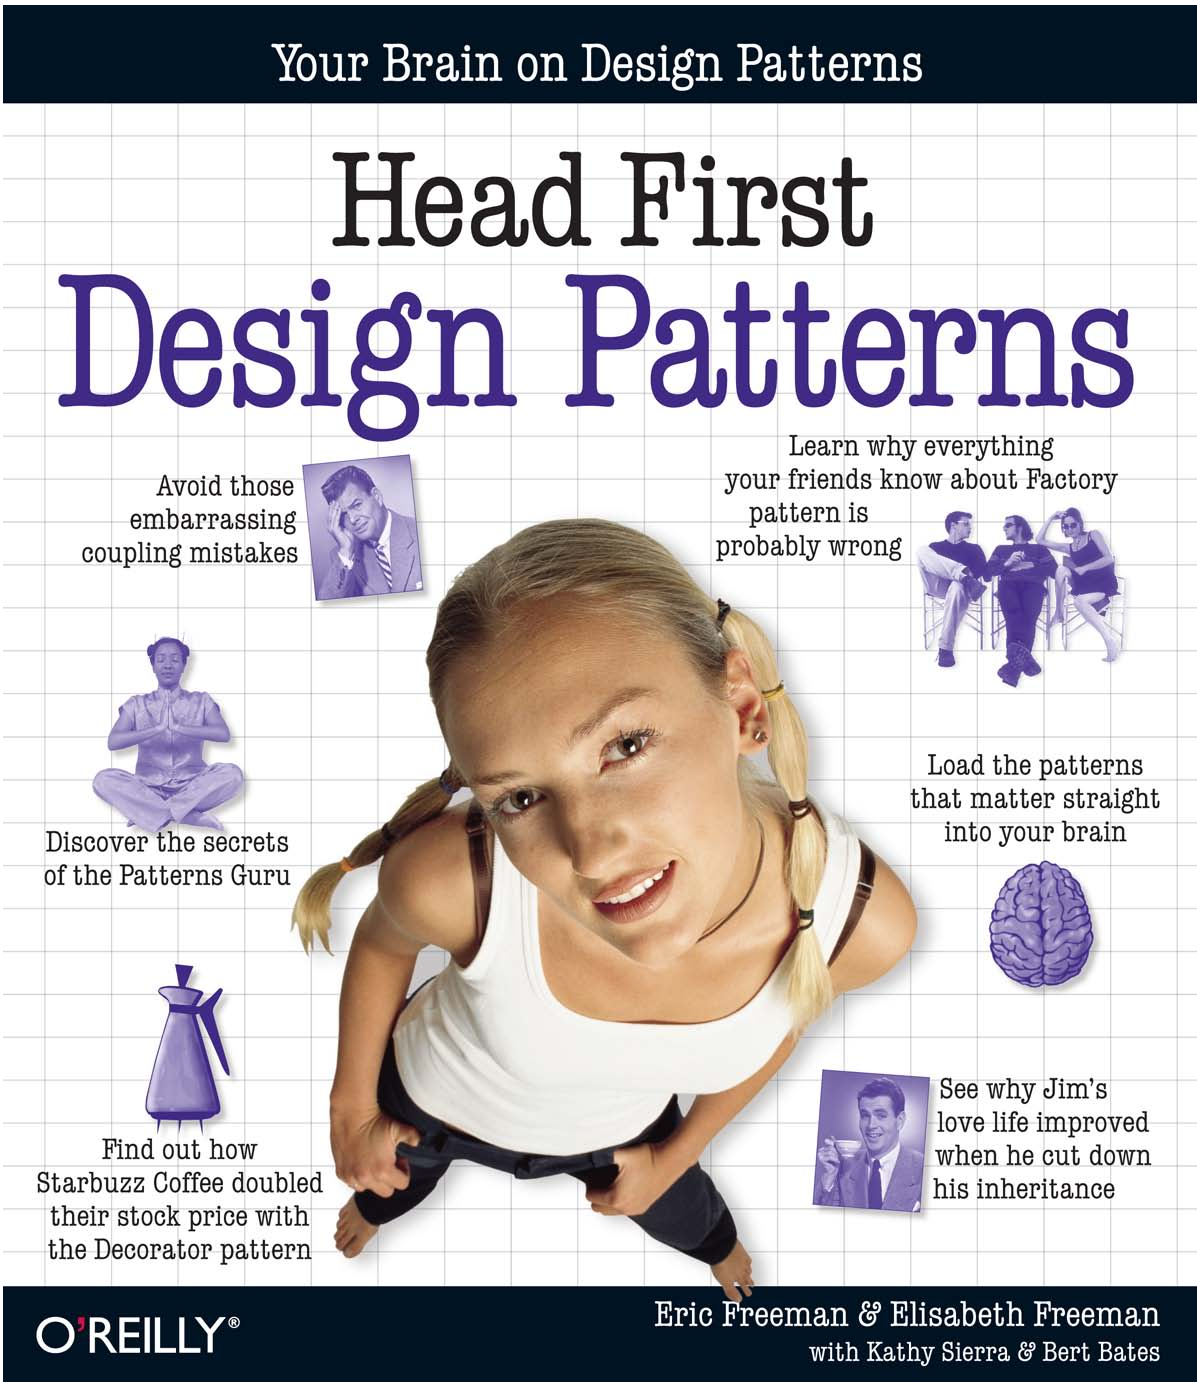
\includegraphics[height=4cm]{headfirstdpcover.pdf}
\end{center}

\end{frame}

\end{document}
